\documentclass[aspectratio=169]{beamer}
\usetheme{metropolis}

%\usepackage{beamerthemesplit}
%\beamertemplatenavigationsymbolsempty
\usepackage{amsmath}
\usepackage{amsthm}
\usepackage{amssymb}
\usepackage{latexsym}
\usepackage{graphicx}
\usepackage{fancybox}
\usepackage{dsfont}
\usepackage{multirow} 
\usepackage{multicol}
\usepackage{booktabs} 
\usepackage{dcolumn}
\usepackage{soul}
%\usepackage[cache=false]{minted}
\usepackage{MnSymbol}
\usepackage{stmaryrd}


\DeclareMathOperator*{\argmax}{arg\,max}
\DeclareMathOperator*{\argmin}{arg\,min}

\newcommand{\X}{\mathtt{X}}
\newcommand{\Y}{\mathtt{Y}}

%\newcommand{\R}{\mathbb{R}}
%\newcommand{\E}{\mathbb{E}}
%\newcommand{\V}{\mathbb{V}}
\newcommand{\p}{\mathbb{P}}
\newcommand*\df{\mathop{}\!\mathrm{d}}
\newcommand{\del}{\partial}


% imports
\usepackage{xargs}
\usepackage{xpatch}
\usepackage{etoolbox}
\usepackage{pdflscape}
\usepackage{booktabs}
\usepackage{threeparttable}
\usepackage[skip=0.2\baselineskip]{caption}

% command for inputting raw latex
\makeatletter
\newcommand\primitiveinput[1]{\@@input #1 }
\makeatother

% common table command
\newcommandx{\tablecontent}[4]{
    \begin{threeparttable}[!ht]
        \centering
        \caption{#3}
        \vspace{-1em}
        \footnotesize
        \begin{tabular}{#1}
            \primitiveinput{../tables/#2.tex}
        \end{tabular}
        \vspace{-0.2em}
        \begin{tablenotes}[flushleft]
            #4
        \end{tablenotes}
    \end{threeparttable}
}




% \usepackage{slashbox}
\title{Lecture 3: Generalized Method of Moments}
\author{Chris Conlon }
\institute{NYU Stern }


\newcommand{\norm}[1]{\left\lVert#1\right\rVert}
\newcommand{\R}{\mathbb{R}}
\newcommand{\E}{\mathbb{E}}
\newcommand{\V}{\mathbb{V}}
\newcommand{\ol}{\overline}
%\newcommand{\ul}{\underline}
\newcommand{\pp}{{\prime \prime}}
\newcommand{\ppp}{{\prime \prime \prime}}
\newcommand{\policy}{\gamma}


\newcommand{\fp}{\frame[plain]}

\date{\today}

\begin{document}
\maketitle



\section{Testing}

\begin{frame}{Testing with MLE}
Before we discuss testing under GMM, let's look at testing under MLE.
\begin{itemize}
\item Helpful to define the \alert{likelihood ratio}
\begin{align*}
LR \equiv -2 \cdot \ln \left[ \frac{\mathcal{L}(\theta_1 | x)}{\mathcal{L}(\theta_2 | x)}  \right]= -2 \cdot \left[ \ell(\theta_1 | x) - \ell(\theta_2 | x) \right]
\end{align*}
\item Consider $\dim(\theta_1) = q_1$ and $\dim(\theta_2) = q_2$ \alert{number of parameters}
\item Often we let $\theta_2$ be the \alert{unrestricted} and $\theta_1$ be the \alert{restricted} model.
\item Define the degrees of \alert{degrees of freedom} $N - \dim(\theta)$.
\item The $LR$ statistic is distributed:
\begin{align*}
 \Lambda \sim \chi^2_{q_1-q_2}
\end{align*}
\item If we know $\theta_1$ and $\theta_2$ and we fix significance level $\alpha =0.05$ then \alert{Neyman-Pearson Lemma} says this is \alert{uniformly post powerful test}.
\end{itemize}
\end{frame}

\begin{frame}{Testing with MLE}
We can consider the more advanced possiblity:
\begin{align*}
L R=-2 \ln \left[\frac{\sup _{\theta \in \Theta_{1}} \mathcal{L}(\theta)}{\sup _{\theta \in \Theta} \mathcal{L}(\theta)}\right]
\end{align*}
\begin{itemize}
\item $\Theta_1$ is a restricted version of the larger set $\Theta$.
\item We can also consider \alert{non nested tests} by looking at differences in \alert{degrees of freedom}
\begin{itemize}
\item This is mostly beyond what we will do in this course.
\item But we could ask: is $x_i$ distributed normally? or log-normally?
\end{itemize}
\end{itemize}
\end{frame}

\begin{frame}{GMM: J-test}
The equivalent test in GMM is the \alert{J-test}
\begin{align*}
Q_N(\theta)&=g_N(\theta)' W_N  g_N(\theta) \\
N \cdot Q_N(\theta) &\rightarrow^D \chi^2_{n-k}
\end{align*}
This is an $LR$-type test statistic.
\end{frame}


\begin{frame}{Inverting LR tests}
A useful technique is that we can always \alert{invert} a test statistic in order to construct confidence intervals.
\begin{itemize}
\item Form an unrestricted estimate $\widehat{\theta}_{MLE}$ or $\widehat{\theta}_{GMM}$
\item Compute $\ell(\widehat{\theta})$.
\item Find all of the $\theta$ such that  $CI=\{\theta: \ell(\widehat{\theta}) -  \ell(\theta) < c \}$.
\item If we do $GMM$ we can use the $J$-stat instead.
\end{itemize}
How to choose $c$ the \alert{critical value}.
\begin{itemize}
\item Compute the number of degrees of freedom / additional restrictions
\item Choose a significance level $\alpha$ (ie: $\alpha=0.05$).
\end{itemize}
\end{frame}


\begin{frame}{Confidence Intervals and Wald Tests}
The multivariate Wald Test is:
\begin{align*}
H_{0}: R \theta=r \quad &
H_{1}: R \theta \neq r\\
\left(R \hat{\theta}_{n}-r\right)^{\prime}\left[R\left(\hat{V}_{n} / n\right) R^{\prime}\right]^{-1}\left(R \hat{\theta}_{n}-r\right) \quad &\rightarrow \quad \chi_{q}^{2}
\end{align*}
\begin{itemize}
\item $R$ is a matrix of $q$ linear restrictions on $k$ parameters.
\item $\hat{V}_n$ is the covariance matrix for $\widehat{\theta}$.
\end{itemize}
You've been constructing CI's this way already
\begin{align*}
\widehat{\beta} \pm 1.96 SE(\widehat{\beta})
\end{align*}
\end{frame}

\begin{frame}{LM or Score Test}
There is a third test known as the \alert{Score Test} or \alert{LM Test}
\begin{align*}
S(\theta)&=\frac{\partial \ell(\theta | x)}{\partial \theta} \\
I(\theta)&=-E\left[\frac{\partial^{2}}{\partial \theta^{2}} \ell(X ; \theta) | \theta\right]
\end{align*}
\begin{itemize}
\item Compute the \alert{score of log likelihood}
\item Compute the \alert{Fisher Information}.
\item The test statistic\
\begin{align*}
S^{T}\left(\hat{\theta}_{0}\right) I^{-1}\left(\hat{\theta}_{0}\right) S\left(\hat{\theta}_{0}\right) \sim \chi_{q}^{2}
\end{align*}
Where $q$ is number of restrictions and $\theta_0$ is the true value.
\end{itemize}
\end{frame}

\begin{frame}{The Trinity of Testing}
\begin{center}
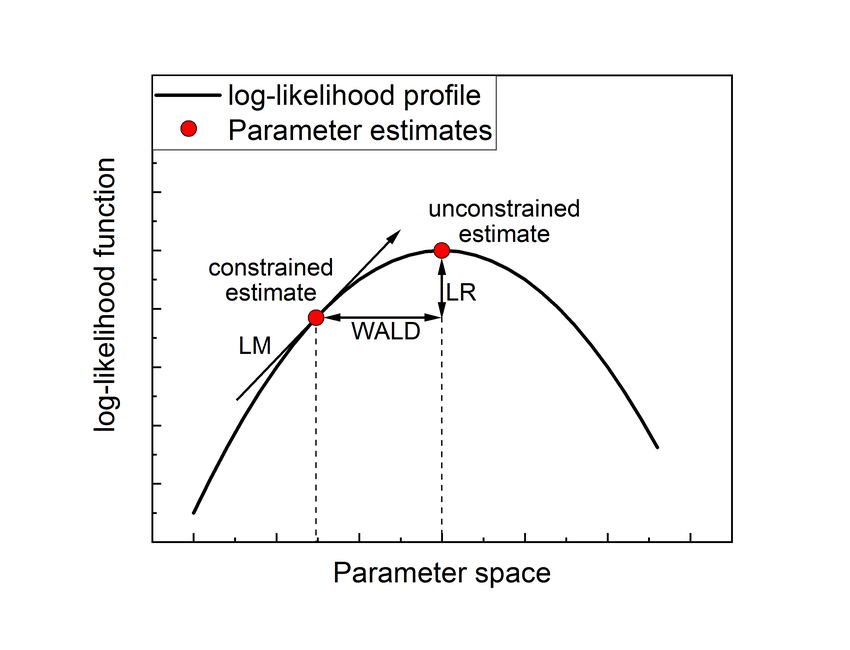
\includegraphics[height=\textheight]{./resources/lmlrwald.png}
\end{center}
\end{frame}

\begin{frame}{What to do in practice?}
\begin{itemize}
\item By reporting asymptotic standard errors you are implicitly using \alert{Wald} type statisitics.
\item If you are comparing models, you should probably try an \alert{LR} type statistic if you can.
\begin{itemize}
\item It used to be people didn't do this because $LR$ required maximizing the objective function more than once.
\item But computers today are pretty good...
\end{itemize}
\item For most extremum estimators (MLE, GMM, GEL, etc.) there are all three kinds of test-statistics
\begin{itemize}
\item ... and around the true $\theta_0$ as $N\rightarrow \infty$ they should coincide.
\item but in finite sample... anything can happen!
\end{itemize}

\end{itemize}

\end{frame}
\section*{Thanks!}

\end{document}